\documentclass[oneside, a4paper,10pt]{report}


 \usepackage[report,tikz,EN]{MyDocumentClass}
% Avaibale Options:
%	OThesis
% 	OReport
%     GLS
% \usepackage{arydshln}
\usepackage[fleqn]{cases}
\usepackage{multirow}
\usepackage{hhline}

\addtolength{\hoffset}{-1cm}
\addtolength{\topmargin}{-2cm}
\addtolength{\textheight}{3cm}
\addtolength{\textwidth}{3cm}


\def\doubleline{
    \vspace{-2.4em}
    
    \noindent\hspace{\fill}\line(1,0){390}\hspace{\fill}
    
    \vspace{-2.4em}
    \noindent\hspace{\fill}\line(1,0){390}\hspace{\fill}
%     \vspace{-2.4em}
%     \hspace{\fill}\line(1,0){340}\hspace{\fill}    
}

% \usepackage{fancyhdr}
%  
% \pagestyle{fancy}
% \lhead{\textbf{Simultaneous Optimization of Parallel Compliance and Damper}}
% \rfoot{ }
% 

\newcommand{\nvar}[2]{%
    \newlength{#1}
    \setlength{#1}{#2}
}


\newcommand{\mc}[2]{\multicolumn{#1}{c}{#2}}
\newcommand{\mr}[2]{\multirow{#1}{*}{#2}}
\newcommand{\Vasat}[2]{\parbox{#1\linewidth}{\centering #2}}
\newcommand{\TR}[1]{\textcolor{red}{#1}}
\newcommand{\TB}[1]{\textcolor{blue}{#1}}
\newcommand{\fr}[1]{\footnotesize{(\hyperref[#1]{+})}}
\newcommand{\BB}[1]{\textit{\textbf{#1}}}


\begin{document} 

{
\small{
\centerline{In the Name of God}}
}


\textbf{\large{General Test Conditions:}}

\bigskip
\bigskip
\centerline{
\begin{tabular}{lllll}
  \noalign{\hrule height 2pt}
  No. of Channels: & 1 to 5  &&
  No. of Subjects: & 109\\ 
  -- & -- &&
  Baseline Channel: & T10 (In case of use)\\
  Task:	& REO &&
  No. of Epochs: & 25\\
  Orthogonal:& Yes (In case of use)&&
  Tries:& 3\\
  Inner Shift: & 4 &&
  Outer Shift: & 8\\
  \noalign{\hrule height 2pt}
\end{tabular}}


\bigskip
\bigskip
\textbf{\large{Overall Test Results:}}

\begin{table}[H]
  \renewcommand{\arraystretch}{1.5}
  \begin{center}
%       \caption{}
      \label{tab:TestResults}
      \begin{tabular}{p{.5cm}|cccc|c|ll|ll|ll}
	  \noalign{\hrule height 2pt}
	  \mr{2}{\rotatebox[origin=c]{90}{\Vasat{.01}{Channels No.}\qquad\quad\quad}} & \mr{2}{\Vasat{.09}{Number of Tries}}& \mr{2}{\Vasat{.1}{Previously Selected Channel(s)}} & \mr{2}{\rotatebox[origin=c]{90}{Baseline}} & \mr{2}{\rotatebox[origin=c]{90}{Orthog.}} & \mr{2}{\Vasat{.1}{Best Channel}}& \mc{2}{Train Data}   & \mc{2}{Validation Data} & \mc{2}{Test Data}\\[.7em]
	  \hhline{~|~~~~|~|--|--|--}
	  % \cmidrule(lr){4-5}\cmidrule(lr){6-7}\cmidrule(lr){8-9}
	  &  &  & & & & Loss & Acc. & Loss & Acc. & Loss & Acc.\\
	  \hhline{-|----|-|--|--|--}
	  \mr{2}{1} & \mr{2}{3} & \mr{2}{-}	& \mr{2}{-} & \mr{2}{$\times$}     & \TB{Oz} (2 out of 3) \fr{fg:1Ch_S109_B0_Avg} 	  & \TB{0.4655} & \TB{0.8514} & \TB{0.5062} & \TB{0.8362} & \TB{0.5059} & \TB{0.8352}\\
		    & 		& 		&   	    &  		           & \TR{Oz} (2 out of 3) \fr{fg:1Ch_S109_B0_Avg}  	  & \TR{0.4724} & \TR{0.8487} & \TR{0.5068} & \TR{0.8344} & \TR{0.5079} & \TR{0.8338}\\
	  \hhline{-|----|-|--|--|--}
	  \mr{4}{2} & \mr{2}{3} & \mr{2}{Oz}	& \mr{2}{-} & \mr{2}{$\checkmark$} & \TB{F8} (0 out of 3) \fr{fg:2Ch_S109_B0_Ort1_Avg} & \TB{0.0617} & \TB{0.9805} & \TB{0.0749} & \TB{0.9748} & \TB{0.0775} & \TB{0.9749}\\
		    & 		& 		& 	    & 			   & \TR{F8} (1 out of 3) \fr{fg:2Ch_S109_B0_Ort1_Avg} & \TR{0.0617} & \TR{0.9805} & \TR{0.0749} & \TR{0.9748} & \TR{0.0775} & \TR{0.9749}\\
	  \hhline{~|----|-|--|--|--}
		    & \mr{2}{3} & \mr{2}{Oz}	& \mr{2}{-} & \mr{2}{$\times$}     & \TB{Fz} (1 out of 3) \fr{fg:2Ch_S109_B0_Ort0_Avg} & \TB{0.1512} & \TB{0.9548} & \TB{0.1838} & \TB{0.9418} & \TB{0.1807} & \TB{0.9433}\\
		    & 		& 		& 	    & 			   & \TR{Fz} (1 out of 3) \fr{fg:2Ch_S109_B0_Ort0_Avg} & \TR{0.1512} & \TR{0.9548} & \TR{0.1838} & \TR{0.9418} & \TR{0.1807} & \TR{0.9433}\\
	  \hhline{-|----|-|--|--|--}
	  \mr{4}{3} & \mr{2}{3} & \mr{2}{Oz, F8}& \mr{2}{-} & \mr{2}{$\checkmark$} & \TB{--} \fr{fg:3Ch_S109_B0_Ort1_Avg} & &&&&&\\%\TB{0.0000} & \TB{0.0000} & \TB{0.0000} & \TB{0.0000} & \TB{0.0000} & \TB{0.0000}\\
		    & 		& 		& 	    & 			   & \TR{--} \fr{fg:3Ch_S109_B0_Ort1_Avg} & &&&&&\\%\TR{0.0000} & \TR{0.0000} & \TR{0.0000} & \TR{0.0000} & \TR{0.0000} & \TR{0.0000}\\
	  \hhline{~|----|-|--|--|--}
		    & \mr{2}{3} & \mr{2}{Oz, Fz}& \mr{2}{-} & \mr{2}{$\times$}     & \TB{--} \fr{fg:3Ch_S109_B0_Ort0_Avg} & &&&&&\\%\TB{0.0000} & \TB{0.0000} & \TB{0.0000} & \TB{0.0000} & \TB{0.0000} & \TB{0.0000}\\
		    & 		& 		& 	    & 			   & \TR{--} \fr{fg:3Ch_S109_B0_Ort0_Avg} & &&&&&\\%\TR{0.0000} & \TR{0.0000} & \TR{0.0000} & \TR{0.0000} & \TR{0.0000} & \TR{0.0000}\\
	  \hhline{~|----|-|--|--|--}
	  \noalign{\hrule height 2pt}
      \end{tabular}
  \end{center}
\end{table}



Description:

\TB{Blue color}: Best Channel according to the train accuracy.

\TR{Red color}: Best Channel according to the test accuracy.

+: Link to the figures and tables in detail.


%%%%%%%%%%%%%%%%%%%%%%%%%%%%%%%%%%%%%%%%%%%%%%%%%%%%%%%%%%%%%%%%%%%%%%%%%%%%%%%%%%%%%%%%%%%%%%%%%%%%%%%%%%%
% SearchSpaceResult_1Ch
\newpage

\hspace*{12cm}\hyperlink{tab:TestResults}{(BACK TO RESULT TABLE)}


\textbf{\large{Case 1 Test Conditions:}}

\bigskip

\centerline{
\begin{tabular}{lllll}
  \noalign{\hrule height 2pt}
  No. of Channels: & 1  &&
  No. of Subjects: & 109\\ 
  Previous Selected Channels: & -- &&
  Baseline Channel: & --\\
  Task:	& REO &&
  No. of Epochs: & 25\\
  Orthogonal:& No.&&
  Tries:& 3\\
  Inner Shift: & 4 &&
  Outer Shift: & 8\\
  \noalign{\hrule height 2pt}
\end{tabular}}

\bigskip

\begin{table}[!hb]
  \renewcommand{\arraystretch}{1.5}
  \begin{center}
      \caption{Avg. Results for Searching first best channel with $109$ subjects, no baseline is removed. Channels are sorted due to the test data accuracy.}
      \label{tab:TestResults}
      \begin{tabular}{c|ll|ll|ll}
	  \noalign{\hrule height 2pt}
	  \mr{2}{\Vasat{.1}{Channel}}& \mc{2}{Train Data}   & \mc{2}{Validation Data} & \mc{2}{Test Data}\\[.7em]
	  \hhline{~|--|--|--}
	  & Loss & Acc. & Loss & Acc. & Loss & Acc.\\
	  \hhline{-|--|--|--}
	  P4,52	&	1.0402	&	0.6749	&	1.0848	&	0.6619	&	1.0916	&	0.6598	\\
	  P3,48	&	0.9958	&	0.6864	&	1.0424	&	0.6734	&	1.0434	&	0.6708	\\
	  Pz,50	&	0.9156	&	0.7207	&	0.9726	&	0.7029	&	0.9715	&	0.7021	\\
	  F7,29	&	0.9033	&	0.7149	&	0.9488	&	0.7034	&	0.9472	&	0.7039	\\
	  P8,54	&	0.9010	&	0.7197	&	0.9443	&	0.7059	&	0.9484	&	0.7056	\\
	  Fp1,21	&	0.8695	&	0.7283	&	0.9234	&	0.7103	&	0.9251	&	0.7117	\\
	  Cz,10	&	0.8564	&	0.7309	&	0.9083	&	0.7171	&	0.9093	&	0.7150	\\
	  C3,8	&	0.8013	&	0.7504	&	0.8514	&	0.7357	&	0.8491	&	0.7352	\\
	  Fp2,23	&	0.7990	&	0.7551	&	0.8465	&	0.7393	&	0.8429	&	0.7402	\\
	  Fz,33	&	0.7587	&	0.7573	&	0.8083	&	0.7431	&	0.8037	&	0.7438	\\
	  T8,41	&	0.7296	&	0.7615	&	0.7619	&	0.7513	&	0.7653	&	0.7493	\\
	  P7,46	&	0.7243	&	0.7653	&	0.7658	&	0.7512	&	0.7685	&	0.7509	\\
	  F3,31	&	0.7160	&	0.7695	&	0.7643	&	0.7542	&	0.7626	&	0.7540	\\
	  F4,35	&	0.7146	&	0.7707	&	0.7539	&	0.7588	&	0.7578	&	0.7573	\\
	  C4,12	&	0.7111	&	0.7783	&	0.7627	&	0.7608	&	0.7712	&	0.7586	\\
	  T7,40	&	0.6517	&	0.7892	&	0.6894	&	0.7793	&	0.6893	&	0.7757	\\
	  F8,36	&	0.6471	&	0.7958	&	0.6889	&	0.7832	&	0.6925	&	0.7802	\\
	  O2,62	&	0.5575	&	0.8189	&	0.5895	&	0.8055	&	0.5958	&	0.8050	\\
	  O1,60	&	0.5302	&	0.8252	&	0.5660	&	0.8137	&	0.5692	&	0.8105	\\
	  Oz,61	&	0.4655	&	0.8514	&	0.5062	&	0.8362	&	0.5059	&	0.8352	\\
	  \noalign{\hrule height 2pt}
      \end{tabular}
  \end{center}
\end{table}

\begin{table}[!h]
  \renewcommand{\arraystretch}{1.5}
  \newcommand{\mcl}[2]{\multicolumn{#1}{|c}{#2}}
  \begin{center}
      \caption{Best channels, in order, in each try.}
      \label{tab:TestResults}
      \begin{tabular}{c|l|p{3cm}|p{3cm}|p{3cm}}
	  \noalign{\hrule height 2pt}
	  \mc{2}{    } 	 	& \mcl{1}{Try 1}   			& \mcl{1}{Try 2} 		& \mcl{1}{Try 3}		\\[.7em]
	  \hhline{-|-|-|-|-}
	  \mr{2}{B.C.} 	& Train & \BB{Oz}$>$O2$>$O1			& \BB{Oz}$>$O2$>$T7		& O1$>$\BB{Oz}$>$O2		\\
	  \hhline{~|-|-|-|-}
			& Test 	& \BB{Oz}$>$O2$>$T7			& \BB{Oz}$>$O2$>$T7		& O1$>$\BB{Oz}$>$O2		\\
	  \noalign{\hrule height 2pt}
      \end{tabular}
  \end{center}
\end{table}

\newpage
\textbf{\large{Case 1 Test Conditions: $^{\text(continued)}$}}

\bigskip
\bigskip

\centerline{
\begin{tabular}{lllll}
  \noalign{\hrule height 2pt}
  No. of Channels: & 1  &&
  No. of Subjects: & 109\\ 
  Previous Selected Channels: & -- &&
  Baseline Channel: & --\\
  Task:	& REO &&
  No. of Epochs: & 25\\
  Orthogonal:& No.&&
  Tries:& 3\\
  Inner Shift: & 4 &&
  Outer Shift: & 8\\
  \noalign{\hrule height 2pt}
\end{tabular}}

\bigskip
\bigskip

\begin{figure}[H]
  \tikzexternaldisable
  \centering
  \begin{tikzpicture}
	  \node[inner sep=0pt] (russell) at (0,0)
	      {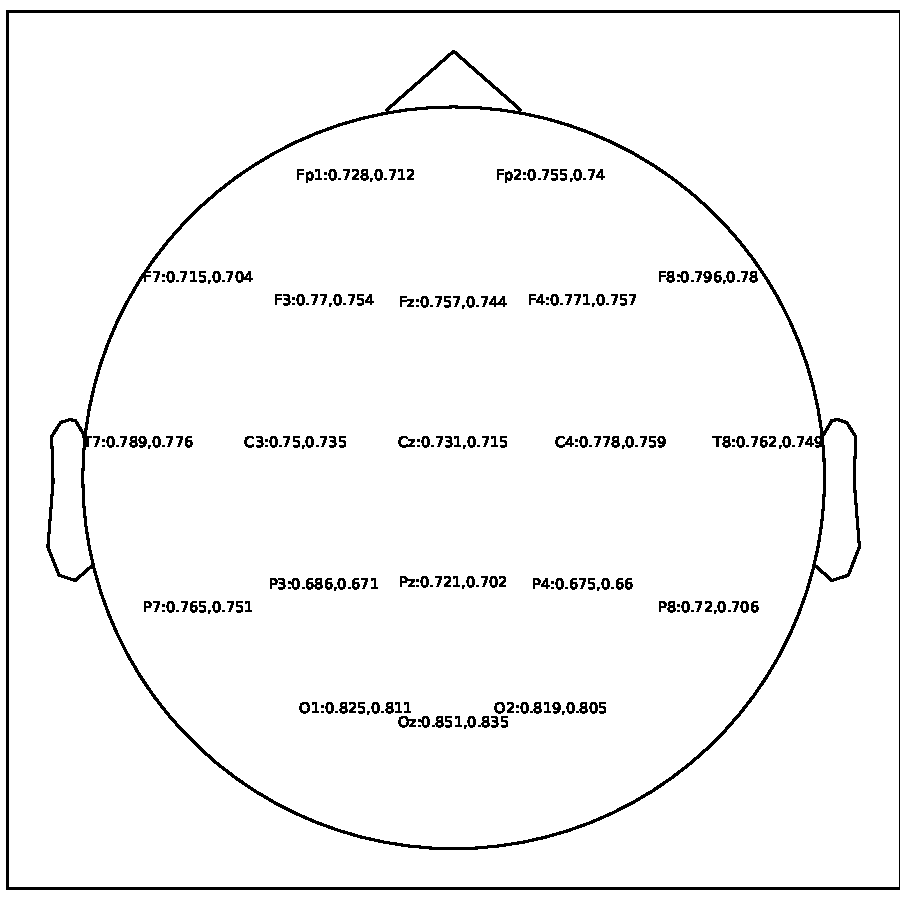
\includegraphics[width=.95\textwidth,trim={0cm 0cm 0cm 0cm},clip]{../SearchResults_1Ch/SearchSpaceResult_1Ch_S109_RemoveBaseLineOff_SamplesIn4Out8_Avg_20191027}};
	  \begin{scope}[scale=1]
	      \draw[line width=2pt,blue] (-7.85,-7.85) node[anchor=west,right=.15cm] {\small{Best Channels according to the train accuracy}} circle (.2);
	      \draw[line width=2pt,red]  (7.85,-7.85)  node[anchor=east,left=.15cm] {\small{Best Channels according to the test accuracy}}  circle (.2);
	      %
	      %\draw[line width=2pt,blue] (-.25,.15) node[] 	(CzTr) {} circle (.45);
	      %\draw[line width=2pt,blue] (-3.2,.15) node[] 	(C3Tr) {} circle (.45);
	      %\draw[line width=2pt,blue] (2.75,.15) node[] 	(C4Tr) {} circle (.45);
	      %\draw[line width=2pt,blue] (-.25, 2.8) node[] 	(FzTr) {} circle (.45);
	      %\draw[line width=2pt,blue] (2.2, 2.85) node[] 	(F4Tr) {} circle (.45);
	      %\draw[line width=2pt,blue] (4.6, 3.25) node[] 	(F8Tr) {} circle (.45);
	      %\draw[line width=2pt,blue] (-2., 5.2) node[] 	(FP1Tr) {} circle (.45);
	      %\draw[line width=2pt,blue] (1.7, 5.2) node[] 	(FP2Tr) {} circle (.45);
	      \draw[line width=2pt,blue] (-.2,-5.1) node[] 	(OzTr) {} circle (.45);
 	      \draw[line width=2pt,blue] (-2.05,-4.85) node[] 	(O1Tr) {} circle (.45);
 	      \draw[line width=2pt,blue] (1.65,-4.85) node[] 	(O2Tr) {} circle (.45);
 	      %\draw[line width=2pt,blue] (-.25, -2.5) node[] 	(PzTr) {} circle (.45);
	      %\draw[line width=2pt,blue] (-2.7, -2.5) node[] 	(P3Tr) {} circle (.45);
	      %\draw[line width=2pt,blue] (-5., -2.95) node[] 	(P7Tr) {} circle (.45);
	      %\draw[line width=2pt,blue] (4.6, -2.95) node[] 	(P8Tr) {} circle (.45);
	      %\draw[line width=2pt,blue] (-6.1,.15) node[] 	(T7Tr) {} circle (.45);
	      %\draw[line width=2pt,blue] (5.75, .15) node[] 	(T8Tr) {} circle (.45);
	      %
	      %\draw[line width=2pt,red] (.65, .15) node[] 	(CzTe) {} circle (.45);
 	      %\draw[line width=2pt,red] (-2.3, .15) node[] 	(C3Te) {} circle (.45);
	      %\draw[line width=2pt,red] (2.8+1, .15) node[] 	(C4Te) {} circle (.45);
	      %\draw[line width=2pt,red] (.6,2.8) node[] 	(FzTe) {} circle (.45);
	      %\draw[line width=2pt,red] (3.1, 2.85) node[] 	(F4Te) {} circle (.45);
	      %\draw[line width=2pt,red] (-4.15, 3.25) node[] 	(F7Te) {} circle (.45);
	      %\draw[line width=2pt,red] (5.45, 3.25) node[] 	(F8Te) {} circle (.45);
	      %\draw[line width=2pt,red] (2.55,5.2) node[] 	(FP2Te) {} circle (.45);
	      \draw[line width=2pt,red] (.7, -5.15) node[] 	(OzTe) {} circle (.45);
	      \draw[line width=2pt,red] (-1.18, -4.85) node[] 	(O1Te) {} circle (.45);
	      \draw[line width=2pt,red] (2.65, -4.85) node[] 	(O2Te) {} circle (.45);
	      %\draw[line width=2pt,red] (.6,-2.5) node[] 	(PzTe) {} circle (.45);
	      %\draw[line width=2pt,red] (3.1,-2.5) node[] 	(P4Te) {} circle (.45);
	      %\draw[line width=2pt,red] (5.45,-2.95) node[] 	(P8Te) {} circle (.45);
	      %\draw[line width=2pt,red] (-5.25, .15) node[] 	(T7Te) {} circle (.45);
 	      %\draw[line width=2pt,red] (6.6, .15) node[] 	(T8Te) {} circle (.45);
	\end{scope}
  \end{tikzpicture}
  \caption{Avg. Results for Searching first best channel with $109$ subjects, no baseline is removed.}
  \label{fg:1Ch_S109_B0_Avg}
\end{figure}

%%%%%%%%%%%%%%%%%%%%%%%%%%%%%%%%%%%%%%%%%%%%%%%%%%%%%%%%%%%%%%%%%%%%%%%%%%%%%%%%%%%%%%%%%%%%%%%%%%%%%%%%%%%
% SearchSpaceResult_2Ch_S109_RemoveBaseLineOff_OrthogonalOn
\newpage

\hspace*{12cm}\hyperlink{tab:TestResults}{(BACK TO RESULT TABLE)}


\textbf{\large{Case 2 Test Conditions:}}

\bigskip

\centerline{
\begin{tabular}{lllll}
  \noalign{\hrule height 2pt}
  No. of Channels: & 2  &&
  No. of Subjects: & 109\\ 
  Previous Selected Channels: & Oz &&
  Baseline Channel: & --\\
  Task:	& REO &&
  No. of Epochs: & 25\\
  Orthogonal:& Yes&&
  Tries:& 3\\
  Inner Shift: & 4 &&
  Outer Shift: & 8\\
  \noalign{\hrule height 2pt}
\end{tabular}}

\bigskip

\begin{table}[!hb]
  \renewcommand{\arraystretch}{1.5}
  \begin{center}
      \caption{Avg. Results for Searching the second best channel with $109$ subjects with orthogonalization. No baseline is removed. Channels are sorted due to the test data accuracy.}
      \label{tab:TestResults}
      \begin{tabular}{c|ll|ll|ll}
	  \noalign{\hrule height 2pt}
	  \mr{2}{\Vasat{.1}{Channel}}& \mc{2}{Train Data}   & \mc{2}{Validation Data} & \mc{2}{Test Data}\\[.7em]
	  \hhline{~|--|--|--}
	  & Loss & Acc. & Loss & Acc. & Loss & Acc.\\
	  \hhline{-|--|--|--}
	  Oz,61	&	0.5181	&	0.8288	&	0.5471	&	0.8178	&	0.5535	&	0.8169	\\
	  T8,41	&	0.1324	&	0.9557	&	0.1573	&	0.9482	&	0.1573	&	0.9475	\\
	  Fp2,23&	0.1206	&	0.9618	&	0.1451	&	0.9519	&	0.1480	&	0.9519	\\
	  P4,52	&	0.1167	&	0.9620	&	0.1380	&	0.9542	&	0.1404	&	0.9535	\\
	  C3,8	&	0.1144	&	0.9650	&	0.1366	&	0.9555	&	0.1384	&	0.9548	\\
	  P3,48	&	0.1062	&	0.9637	&	0.1255	&	0.9565	&	0.1258	&	0.9567	\\
	  O1,60	&	0.1092	&	0.9650	&	0.1290	&	0.9574	&	0.1297	&	0.9574	\\
	  Pz,50	&	0.1107	&	0.9639	&	0.1279	&	0.9579	&	0.1267	&	0.9585	\\
	  Fp1,21&	0.0998	&	0.9686	&	0.1180	&	0.9620	&	0.1216	&	0.9607	\\
	  C4,12	&	0.0901	&	0.9718	&	0.1106	&	0.9634	&	0.1131	&	0.9622	\\
	  Cz,10	&	0.0912	&	0.9706	&	0.1102	&	0.9631	&	0.1112	&	0.9629	\\
	  F3,31	&	0.0876	&	0.9728	&	0.1080	&	0.9648	&	0.1109	&	0.9636	\\
	  T7,40	&	0.0887	&	0.9724	&	0.1069	&	0.9668	&	0.1107	&	0.9639	\\
	  F7,29	&	0.0866	&	0.9725	&	0.1017	&	0.9665	&	0.1083	&	0.9648	\\
	  O2,62	&	0.0893	&	0.9722	&	0.1086	&	0.9657	&	0.1095	&	0.9652	\\
	  P7,46	&	0.0839	&	0.9728	&	0.1018	&	0.9663	&	0.1017	&	0.9661	\\
	  F4,35	&	0.0774	&	0.9760	&	0.1000	&	0.9668	&	0.1025	&	0.9668	\\
	  Fz,33	&	0.0754	&	0.9770	&	0.0933	&	0.9702	&	0.0976	&	0.9687	\\
	  P8,54	&	0.0702	&	0.9794	&	0.0886	&	0.9726	&	0.0895	&	0.9722	\\
	  F8,36	&	0.0617	&	0.9805	&	0.0749	&	0.9748	&	0.0775	&	0.9749	\\
	  \noalign{\hrule height 2pt}
      \end{tabular}
  \end{center}
\end{table}

\begin{table}[!h]
  \renewcommand{\arraystretch}{1.5}
  \newcommand{\mcl}[2]{\multicolumn{#1}{|c}{#2}}
  \begin{center}
      \caption{Best channels, in order, in each try.}
      \label{tab:TestResults}
      \begin{tabular}{c|l|p{3cm}|p{3cm}|p{3cm}}
	  \noalign{\hrule height 2pt}
	  \mc{2}{    } 	 	& \mcl{1}{Try 1}   			& \mcl{1}{Try 2} 		& \mcl{1}{Try 3}			\\[.7em]
	  \hhline{-|-|-|-|-}
	  \mr{2}{B.C.} 	& Train & Fz$>$F7$>$Fp1$>$\BB{F8}		& O2$>$P3$>$\BB{F8}		& F7$>$O2$>$\BB{F8}		\\
	  \hhline{~|-|-|-|-}
			& Test 	& F7$>$Fz$>$\BB{F8}			& O2$>$\BB{F8}$>$P3		& \BB{F8}$>$F7$>$P8		\\
	  \noalign{\hrule height 2pt}
      \end{tabular}
  \end{center}
\end{table}

\newpage
\textbf{\large{Case 2 Test Conditions: $^{\text(continued)}$}}

\bigskip
\bigskip

\centerline{
\begin{tabular}{lllll}
  \noalign{\hrule height 2pt}
  No. of Channels: & 2  &&
  No. of Subjects: & 109\\ 
  Previous Selected Channels: & Oz &&
  Baseline Channel: & --\\
  Task:	& REO &&
  No. of Epochs: & 25\\
  Orthogonal:& Yes&&
  Tries:& 3\\
  Inner Shift: & 4 &&
  Outer Shift: & 8\\
  \noalign{\hrule height 2pt}
\end{tabular}}

\bigskip
\bigskip

\begin{figure}[H]
  \tikzexternaldisable
  \centering
  \begin{tikzpicture}
	  \node[inner sep=0pt] (russell) at (0,0)
	      {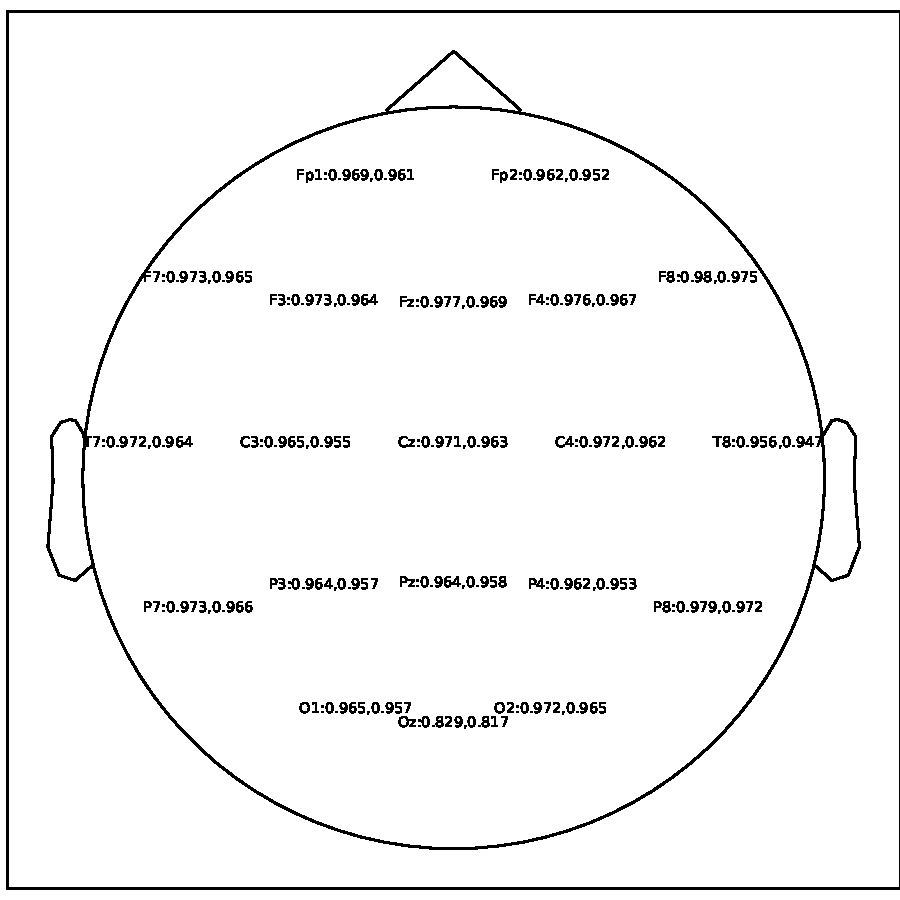
\includegraphics[width=.95\textwidth,trim={0cm 0cm 0cm 0cm},clip]{../SearchResults_2Ch/SearchSpaceResult_2Ch_(61)_S109_RemoveBaseLineOff_OrthogonalOn_SamplesIn4Out8_Avg_20191027}};
	  \begin{scope}[scale=1]
	      \draw[line width=2pt,blue] (-7.85,-7.85) node[anchor=west,right=.15cm] {\small{Best Channels according to the train accuracy}} circle (.2);
	      \draw[line width=2pt,red]  (7.85,-7.85)  node[anchor=east,left=.15cm] {\small{Best Channels according to the test accuracy}}  circle (.2);
	      \draw[line width=2pt,green,fill=green] (-7.85,7.85) node[anchor=west,right=.15cm,opacity=1] {{Previously Selected Channels}} circle (.25);
 	      %
	      \draw[line width=2pt,green,fill=green,opacity=.5] (-.82,-5.15) node[] 	(OzPS) {} circle (.25);
 	      %
	      %\draw[line width=2pt,blue] (-.25,.15) node[] 	(CzTr) {} circle (.45);
	      %\draw[line width=2pt,blue] (-3.2,.15) node[] 	(C3Tr) {} circle (.45);
	      %\draw[line width=2pt,blue] (2.75,.15) node[] 	(C4Tr) {} circle (.45);
	      \draw[line width=2pt,blue] (-.2, 2.8) node[] 	(FzTr) {} circle (.45);
	      %\draw[line width=2pt,blue] (2.2, 2.85) node[] 	(F4Tr) {} circle (.45);
	      \draw[line width=2pt,blue] (4.75, 3.25) node[] 	(F8Tr) {} circle (.45);
	      %\draw[line width=2pt,blue] (-2., 5.2) node[] 	(FP1Tr) {} circle (.45);
	      %\draw[line width=2pt,blue] (1.7, 5.2) node[] 	(FP2Tr) {} circle (.45);
	      %\draw[line width=2pt,blue] (-.2,-5.1) node[] 	(OzTr) {} circle (.45);
 	      %\draw[line width=2pt,blue] (-2.05,-4.85) node[] 	(O1Tr) {} circle (.45);
 	      %\draw[line width=2pt,blue] (1.65,-4.85) node[] 	(O2Tr) {} circle (.45);
 	      %\draw[line width=2pt,blue] (-.25, -2.5) node[] 	(PzTr) {} circle (.45);
	      %\draw[line width=2pt,blue] (-2.7, -2.5) node[] 	(P3Tr) {} circle (.45);
	      %\draw[line width=2pt,blue] (-5., -2.95) node[] 	(P7Tr) {} circle (.45);
	      \draw[line width=2pt,blue] (4.7, -2.95) node[] 	(P8Tr) {} circle (.45);
	      %\draw[line width=2pt,blue] (-6.1,.15) node[] 	(T7Tr) {} circle (.45);
	      %\draw[line width=2pt,blue] (5.75, .15) node[] 	(T8Tr) {} circle (.45);
	      %
	      %\draw[line width=2pt,red] (.65, .15) node[] 	(CzTe) {} circle (.45);
 	      %\draw[line width=2pt,red] (-2.3, .15) node[] 	(C3Te) {} circle (.45);
	      %\draw[line width=2pt,red] (2.8+1, .15) node[] 	(C4Te) {} circle (.45);
	      \draw[line width=2pt,red] (.65,2.8) node[] 	(FzTe) {} circle (.45);
	      %\draw[line width=2pt,red] (3.1, 2.85) node[] 	(F4Te) {} circle (.45);
	      %\draw[line width=2pt,red] (-4.15, 3.25) node[] 	(F7Te) {} circle (.45);
	      \draw[line width=2pt,red] (5.55, 3.25) node[] 	(F8Te) {} circle (.45);
	      %\draw[line width=2pt,red] (2.55,5.2) node[] 	(FP2Te) {} circle (.45);
	      %\draw[line width=2pt,red] (.7, -5.15) node[] 	(OzTe) {} circle (.45);
	      %\draw[line width=2pt,red] (-1.18, -4.85) node[] 	(O1Te) {} circle (.45);
	      %\draw[line width=2pt,red] (2.65, -4.85) node[] 	(O2Te) {} circle (.45);
	      %\draw[line width=2pt,red] (.6,-2.5) node[] 	(PzTe) {} circle (.45);
	      %\draw[line width=2pt,red] (3.1,-2.5) node[] 	(P4Te) {} circle (.45);
	      \draw[line width=2pt,red] (5.55,-2.95) node[] 	(P8Te) {} circle (.45);
	      %\draw[line width=2pt,red] (-5.25, .15) node[] 	(T7Te) {} circle (.45);
 	      %\draw[line width=2pt,red] (6.6, .15) node[] 	(T8Te) {} circle (.45);
	\end{scope}
  \end{tikzpicture}
  \caption{Avg. Results for Searching the second best channel with $109$ subjects with orthogonalization. No baseline is removed.}
  \label{fg:2Ch_S109_B0_Ort1_Avg}
\end{figure}

%%%%%%%%%%%%%%%%%%%%%%%%%%%%%%%%%%%%%%%%%%%%%%%%%%%%%%%%%%%%%%%%%%%%%%%%%%%%%%%%%%%%%%%%%%%%%%%%%%%%%%%%%%%
% SearchSpaceResult_2Ch_S109_RemoveBaseLineOff_OrthogonalOff
\newpage

\hspace*{12cm}\hyperlink{tab:TestResults}{(BACK TO RESULT TABLE)}


\textbf{\large{Case 3 Test Conditions:}}

\bigskip

\centerline{
\begin{tabular}{lllll}
  \noalign{\hrule height 2pt}
  No. of Channels: & 2  &&
  No. of Subjects: & 109\\ 
  Previous Selected Channels: & Oz &&
  Baseline Channel: & --\\
  Task:	& REO &&
  No. of Epochs: & 25\\
  Orthogonal:& No&&
  Tries:& 3\\
  Inner Shift: & 4 &&
  Outer Shift: & 8\\
  \noalign{\hrule height 2pt}
\end{tabular}}

\bigskip

\begin{table}[!h]
  \renewcommand{\arraystretch}{1.5}
  \begin{center}
      \caption{Avg. Results for Searching the second best channel with $109$ subjects without orthogonalization. No baseline is removed. Channels are sorted due to the test data accuracy.}
      \label{tab:TestResults}
      \begin{tabular}{c|ll|ll|ll}
	  \noalign{\hrule height 2pt}
	  \mr{2}{\Vasat{.1}{Channel}}& \mc{2}{Train Data}   & \mc{2}{Validation Data} & \mc{2}{Test Data}\\[.7em]
	  \hhline{~|--|--|--}
	  & Loss & Acc. & Loss & Acc. & Loss & Acc.\\
	  \hhline{-|--|--|--}
	  Oz,61	&	0.4567	&	0.8518	&	0.5041	&	0.8344	&	0.5049	&	0.8342	\\
	  C4,12	&	0.3048	&	0.9015	&	0.3435	&	0.8895	&	0.3474	&	0.8878	\\
	  P7,46	&	0.2696	&	0.9148	&	0.3034	&	0.9018	&	0.3095	&	0.8998	\\
	  T7,40	&	0.2629	&	0.9131	&	0.2922	&	0.9050	&	0.2941	&	0.9031	\\
	  Cz,10	&	0.2610	&	0.9148	&	0.2951	&	0.9037	&	0.2958	&	0.9032	\\
	  Fp2,23&	0.2551	&	0.9196	&	0.3056	&	0.9017	&	0.3076	&	0.9037	\\
	  Pz,50	&	0.2668	&	0.9170	&	0.3019	&	0.9052	&	0.3013	&	0.9044	\\
	  Fp1,21&	0.2535	&	0.9247	&	0.3078	&	0.9057	&	0.3089	&	0.9061	\\
	  C3,8	&	0.2578	&	0.9192	&	0.2900	&	0.9080	&	0.2925	&	0.9075	\\
	  F7,29	&	0.2419	&	0.9247	&	0.2865	&	0.9094	&	0.2876	&	0.9089	\\
	  O1,60	&	0.2408	&	0.9236	&	0.2719	&	0.9114	&	0.2700	&	0.9128	\\
	  P8,54	&	0.2389	&	0.9265	&	0.2729	&	0.9134	&	0.2711	&	0.9153	\\
	  F3,31	&	0.2124	&	0.9305	&	0.2542	&	0.9164	&	0.2539	&	0.9168	\\
	  P4,52	&	0.2213	&	0.9353	&	0.2541	&	0.9227	&	0.2562	&	0.9202	\\
	  F4,35	&	0.1900	&	0.9399	&	0.2265	&	0.9270	&	0.2260	&	0.9260	\\
	  P3,48	&	0.2037	&	0.9386	&	0.2335	&	0.9273	&	0.2346	&	0.9270	\\
	  O2,62	&	0.1943	&	0.9390	&	0.2246	&	0.9275	&	0.2241	&	0.9278	\\
	  F8,36	&	0.1942	&	0.9432	&	0.2284	&	0.9300	&	0.2320	&	0.9297	\\
	  T8,41	&	0.1788	&	0.9497	&	0.2094	&	0.9380	&	0.2096	&	0.9387	\\
	  Fz,33	&	0.1512	&	0.9548	&	0.1838	&	0.9418	&	0.1807	&	0.9433	\\
	  \noalign{\hrule height 2pt}
      \end{tabular}
  \end{center}
\end{table}

\begin{table}[!h]
  \renewcommand{\arraystretch}{1.5}
  \newcommand{\mcl}[2]{\multicolumn{#1}{|c}{#2}}
  \begin{center}
      \caption{Best channels, in order, in each try.}
      \label{tab:TestResults}
      \begin{tabular}{c|l|p{4.5cm}|p{4cm}|p{4cm}}
	  \noalign{\hrule height 2pt}
	  \mc{2}{    } 	 	& \mcl{1}{Try 1}   			& \mcl{1}{Try 2} 		& \mcl{1}{Try 3}			\\[.7em]
	  \hhline{-|-|-|-|-}
	  \mr{2}{B.C.} 	& Train & T7$>$Fp2$>$F4$>$P8$>$Fp1$>$\BB{Fz}	& F4$>$T8$>$\BB{Fz}		& \BB{Fz}$>$P3$>$P7		\\
	  \hhline{~|-|-|-|-}
			& Test 	& T7$>$Fp2$>$P8$>$\BB{Fz}		& F4$>$T8$>$F7$>$\BB{Fz}	& \BB{Fz}$>$P3$>$F3		\\
	  \noalign{\hrule height 2pt}
      \end{tabular}
  \end{center}
\end{table}

\newpage
\textbf{\large{Case 3 Test Conditions: $^{\text(continued)}$}}

\bigskip
\bigskip

\centerline{
\begin{tabular}{lllll}
  \noalign{\hrule height 2pt}
  No. of Channels: & 2  &&
  No. of Subjects: & 109\\ 
  Previous Selected Channels: & Oz &&
  Baseline Channel: & --\\
  Task:	& REO &&
  No. of Epochs: & 25\\
  Orthogonal:& No&&
  Tries:& 3\\
  Inner Shift: & 4 &&
  Outer Shift: & 8\\
  \noalign{\hrule height 2pt}
\end{tabular}}

\bigskip
\bigskip

\begin{figure}[H]
  \tikzexternaldisable
  \centering
  \begin{tikzpicture}
	  \node[inner sep=0pt] (russell) at (0,0)
	      {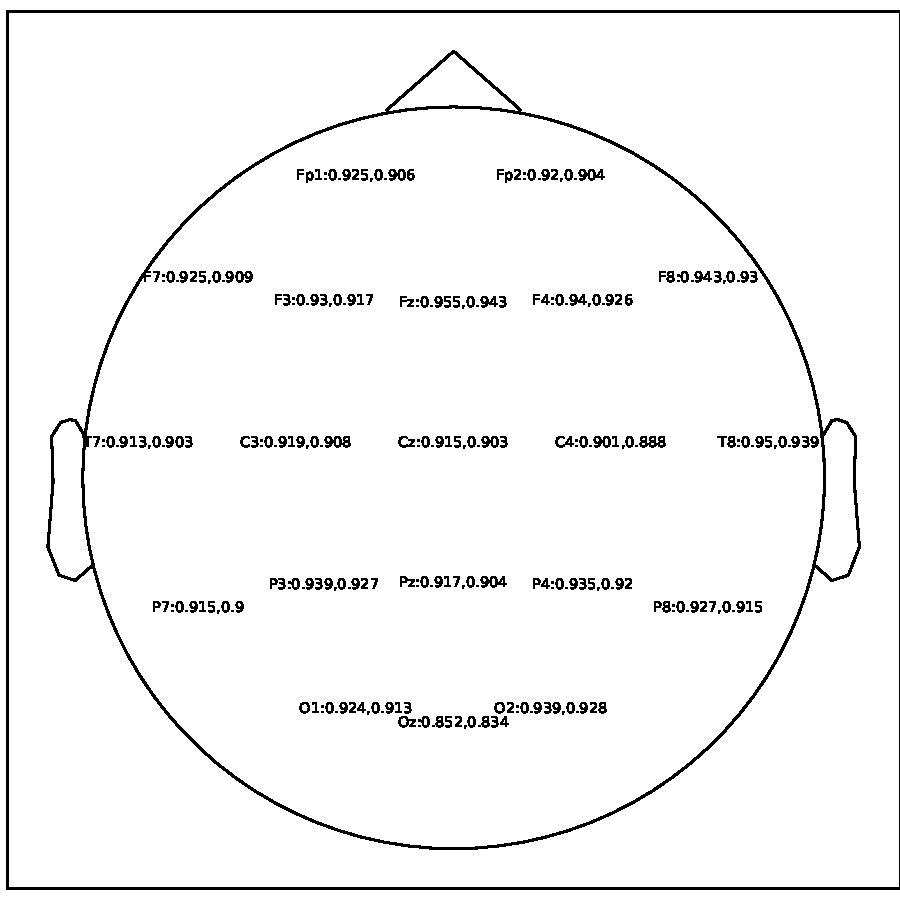
\includegraphics[width=.95\textwidth,trim={0cm 0cm 0cm 0cm},clip]{../SearchResults_2Ch/SearchSpaceResult_2Ch_(61)_S109_RemoveBaseLineOff_OrthogonalOff_SamplesIn4Out8_Avg_20191028}};
	  \begin{scope}[scale=1]
	      \draw[line width=2pt,blue] (-7.85,-7.85) node[anchor=west,right=.15cm] {\small{Best Channels according to the train accuracy}} circle (.2);
	      \draw[line width=2pt,red]  (7.85,-7.85)  node[anchor=east,left=.15cm] {\small{Best Channels according to the test accuracy}}  circle (.2);
	      \draw[line width=2pt,green,fill=green] (-7.85,7.85) node[anchor=west,right=.15cm,opacity=1] {{Previously Selected Channels}} circle (.25);
 	      %
	      \draw[line width=2pt,green,fill=green,opacity=.5] (-.82,-5.15) node[] 	(OzPS) {} circle (.25);
 	      %
	      %\draw[line width=2pt,blue] (-.25,.15) node[] 	(CzTr) {} circle (.45);
	      %\draw[line width=2pt,blue] (-3.2,.15) node[] 	(C3Tr) {} circle (.45);
	      %\draw[line width=2pt,blue] (2.75,.15) node[] 	(C4Tr) {} circle (.45);
	      \draw[line width=2pt,blue] (-.2, 2.8) node[] 	(FzTr) {} circle (.45);
	      %\draw[line width=2pt,blue] (2.2, 2.85) node[] 	(F4Tr) {} circle (.45);
	      \draw[line width=2pt,blue] (4.75, 3.25) node[] 	(F8Tr) {} circle (.45);
	      %\draw[line width=2pt,blue] (-2., 5.2) node[] 	(FP1Tr) {} circle (.45);
	      %\draw[line width=2pt,blue] (1.7, 5.2) node[] 	(FP2Tr) {} circle (.45);
	      %\draw[line width=2pt,blue] (-.2,-5.1) node[] 	(OzTr) {} circle (.45);
 	      %\draw[line width=2pt,blue] (-2.05,-4.85) node[] 	(O1Tr) {} circle (.45);
 	      %\draw[line width=2pt,blue] (1.65,-4.85) node[] 	(O2Tr) {} circle (.45);
 	      %\draw[line width=2pt,blue] (-.25, -2.5) node[] 	(PzTr) {} circle (.45);
	      %\draw[line width=2pt,blue] (-2.7, -2.5) node[] 	(P3Tr) {} circle (.45);
	      %\draw[line width=2pt,blue] (-5., -2.95) node[] 	(P7Tr) {} circle (.45);
	      %\draw[line width=2pt,blue] (4.7, -2.95) node[] 	(P8Tr) {} circle (.45);
	      %\draw[line width=2pt,blue] (-6.1,.15) node[] 	(T7Tr) {} circle (.45);
	      \draw[line width=2pt,blue] (5.75, .15) node[] 	(T8Tr) {} circle (.45);
	      %
	      %\draw[line width=2pt,red] (.65, .15) node[] 	(CzTe) {} circle (.45);
 	      %\draw[line width=2pt,red] (-2.3, .15) node[] 	(C3Te) {} circle (.45);
	      %\draw[line width=2pt,red] (2.8+1, .15) node[] 	(C4Te) {} circle (.45);
	      \draw[line width=2pt,red] (.65,2.8) node[] 	(FzTe) {} circle (.45);
	      %\draw[line width=2pt,red] (3.1, 2.85) node[] 	(F4Te) {} circle (.45);
	      %\draw[line width=2pt,red] (-4.15, 3.25) node[] 	(F7Te) {} circle (.45);
	      \draw[line width=2pt,red] (5.6, 3.25) node[] 	(F8Te) {} circle (.45);
	      %\draw[line width=2pt,red] (2.55,5.2) node[] 	(FP2Te) {} circle (.45);
	      %\draw[line width=2pt,red] (.7, -5.15) node[] 	(OzTe) {} circle (.45);
	      %\draw[line width=2pt,red] (-1.18, -4.85) node[] 	(O1Te) {} circle (.45);
	      %\draw[line width=2pt,red] (2.65, -4.85) node[] 	(O2Te) {} circle (.45);
	      %\draw[line width=2pt,red] (.6,-2.5) node[] 	(PzTe) {} circle (.45);
	      %\draw[line width=2pt,red] (3.1,-2.5) node[] 	(P4Te) {} circle (.45);
	      %\draw[line width=2pt,red] (5.55,-2.95) node[] 	(P8Te) {} circle (.45);
	      %\draw[line width=2pt,red] (-5.25, .15) node[] 	(T7Te) {} circle (.45);
 	      \draw[line width=2pt,red] (6.6, .15) node[] 	(T8Te) {} circle (.45);
	\end{scope}
  \end{tikzpicture}
  \caption{Avg. Results for Searching the second best channel with $109$ subjects without orthogonalization. No baseline is removed.}
  \label{fg:2Ch_S109_B0_Ort0_Avg}
\end{figure}





\end{document}